% Importado desde: 2026-03-28_Isotropia_y_Simetrias_en_QW_3D_Weyl.tex
\chapter{Derivacion Pedagogica: --- isotropia y estructura de simetrias --- en una quantum walk concreta \(3D\) tipo Weyl}
\label{ch:isotropia-qw-3d-weyl}

\section{Objetivo}
En el capitulo anterior vimos en \(2D\) una leccion muy importante: una dinamica discreta local puede ser microscópicamente anisotropa y, sin embargo, recombinarse en un sector infrarrojo isotropo.

Ahora queremos repetir la pregunta en \(3D\), pero ya no con una caminata de tipo Dirac completa, sino con su bloque minimo mas natural:
\begin{displayquote}
\textbf{una quantum walk discreta cuyo limite efectivo sea un Hamiltoniano de Weyl en tres dimensiones.}
\end{displayquote}

Las preguntas centrales de este capitulo son:
\begin{enumerate}[label=\arabic*.]
    \item cual es la construccion minima concreta en \(3D\);
    \item por que su limite infrarrojo es isotropo;
    \item que simetrias tiene realmente a nivel microscopico;
    \item y que falta todavia para pasar de Weyl a Dirac en \(3+1\).
\end{enumerate}

\section{La caminata minima en \(3D\)}
\subsection{Idea de partida}
La version mas sobria del paso unitario consiste en tomar tres subpasos, uno por cada eje cartesiano:
\begin{equation}
U_W = U_z\,U_y\,U_x,
\label{c09:eq:UW}
\end{equation}
con
\begin{equation}
U_x = \ee^{-\,\ii a p_x \sigma_x},
\qquad
U_y = \ee^{-\,\ii a p_y \sigma_y},
\qquad
U_z = \ee^{-\,\ii a p_z \sigma_z}.
\label{c09:eq:substeps}
\end{equation}

Aqui:
\begin{enumerate}[label=\arabic*.]
    \item \(a\) es la longitud elemental del paso espacial;
    \item \(p_i=-\ii \partial_i\);
    \item cada direccion espacial viene acompa\~nada por una matriz de Pauli distinta.
\end{enumerate}

\subsection{Lectura fisica}
La estructura del modelo es muy natural:
\begin{enumerate}[label=\arabic*.]
    \item el espacio interno tiene dos componentes;
    \item cada subpaso vincula una direccion espacial con una direccion en el espacio de Pauli;
    \item la composicion total esta dise\~nada para reconstruir un bloque tipo Weyl.
\end{enumerate}

\begin{figure}[h!]
\centering
\begin{tikzpicture}[>=Latex,node distance=1.15cm]
  \node[draw,rounded corners,fill=blue!7,minimum width=2.2cm,minimum height=0.85cm] (x) {\(U_x\)};
  \node[draw,rounded corners,fill=blue!7,minimum width=2.2cm,minimum height=0.85cm,right=of x] (y) {\(U_y\)};
  \node[draw,rounded corners,fill=blue!7,minimum width=2.2cm,minimum height=0.85cm,right=of y] (z) {\(U_z\)};
  \draw[->,thick] (x) -- (y);
  \draw[->,thick] (y) -- (z);
  \node[below=0.55cm of y] {\small tres subpasos espaciales con estructura interna};
\end{tikzpicture}
\caption{La quantum walk minima \(3D\) tipo Weyl.}
\end{figure}

\section{Primer analisis: el limite efectivo}
\subsection{Expansion a primer orden}
Para momentos pequenos, \(a|\vp|\ll 1\), expandimos cada factor:
\begin{equation}
U_i \simeq \bbI - \ii a p_i \sigma_i.
\end{equation}

Entonces:
\begin{equation}
U_W
\simeq
\left(\bbI-\ii a p_z \sigma_z\right)
\left(\bbI-\ii a p_y \sigma_y\right)
\left(\bbI-\ii a p_x \sigma_x\right).
\end{equation}

Reteniendo solo primer orden:
\begin{equation}
U_W \simeq \bbI - \ii a\left(p_x \sigma_x + p_y \sigma_y + p_z \sigma_z\right).
\label{c09:eq:UWexp}
\end{equation}

Por otro lado,
\begin{equation}
U_W \simeq \bbI - \ii \Delta t\,H_{\text{eff}}.
\end{equation}

Comparando ambas expresiones:
\begin{equation}
H_{\text{eff}}
=
\frac{a}{\Delta t}\left(p_x \sigma_x + p_y \sigma_y + p_z \sigma_z\right).
\end{equation}

Definiendo
\begin{equation}
v=\frac{a}{\Delta t},
\end{equation}
queda
\begin{equation}
H_{\text{eff}} = v\left(\sigma_x p_x + \sigma_y p_y + \sigma_z p_z\right).
\label{c09:eq:WeylEff}
\end{equation}

Este es precisamente el Hamiltoniano de Weyl que queriamos.

\subsection{Espectro}
El espectro es
\begin{equation}
E_\pm(\vp)=\pm v\sqrt{p_x^2+p_y^2+p_z^2}.
\label{c09:eq:disp}
\end{equation}

Las superficies de energia constante satisfacen
\begin{equation}
p_x^2+p_y^2+p_z^2 = \text{constante},
\end{equation}
o sea: son esferas en el espacio de momentos.

\section{Por que esto ya implica isotropia efectiva}
El modelo microscópico distingue claramente los ejes \(x,y,z\). Pero el espectro \eqref{c09:eq:disp} solo depende de
\begin{equation}
\abs{\vp}^2 = p_x^2+p_y^2+p_z^2.
\end{equation}

Eso significa que la dinamica infrarroja ya no recuerda la diferencia entre los tres ejes. A primer orden, solo queda una velocidad comun \(v\).

\subsection{Leccion fuerte}
La leccion es la misma que en \(2D\), pero ahora en una version mas poderosa:
\begin{displayquote}
\textbf{la estructura discreta cartesiana puede reorganizarse en un cono de Weyl completamente isotropo en el limite de baja energia.}
\end{displayquote}

\begin{figure}[h!]
\centering
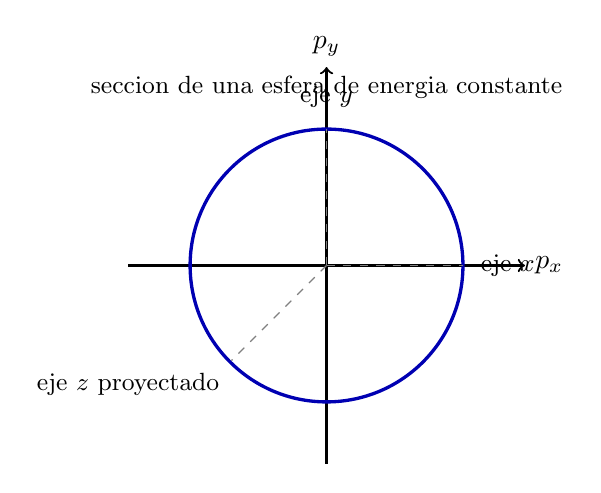
\begin{tikzpicture}[scale=1.05]
  \draw[->,thick] (-2.4,0) -- (2.4,0) node[right] {\(p_x\)};
  \draw[->,thick] (0,-2.4) -- (0,2.4) node[above] {\(p_y\)};
  \draw[very thick,blue!70!black] (0,0) circle (1.65);
  \draw[gray,dashed] (0,0) -- (1.65,0);
  \draw[gray,dashed] (0,0) -- (0,1.65);
  \draw[gray,dashed] (0,0) -- (-1.15,-1.15);
  \node[right] at (1.75,0) {\small eje \(x\)};
  \node[above] at (0,1.8) {\small eje \(y\)};
  \node[below left] at (-1.18,-1.18) {\small eje \(z\) proyectado};
  \node at (0,2.15) {\small seccion de una esfera de energia constante};
\end{tikzpicture}
\caption{Aunque la caminata usa tres ejes distinguidos, la dispersion efectiva depende solo de \(\abs{\vp}\).}
\end{figure}

\section{Segundo analisis: las simetrias microscopicas}
\subsection{Traslaciones discretas}
La primera simetria exacta es la invariancia por traslaciones de la red cubica. El paso local es el mismo en todas las celdas.

\subsection{Simetria de la red y advertencia sobre el paso}
La geometria de la red cubica sugiere naturalmente simetrias puntuales discretas. Microscopicamente no tenemos \(SO(3)\), sino una estructura de red con ejes privilegiados.

Pero aqui hay que introducir una advertencia importante. Nuestra caminata minima esta escrita como un producto ordenado de subpasos,
\begin{equation}
U_W = U_z\,U_y\,U_x,
\end{equation}
y ese orden deja memoria microscopica. Por eso no toda simetria de la red tiene por que sobrevivir como simetria exacta del paso completo.

Para no dispersarnos, basta analizar un generador sencillo a nivel del bloque linealizado: la rotacion espacial de \(\pi/2\) alrededor del eje \(z\):
\begin{equation}
R_z\left(\frac{\pi}{2}\right):
\qquad
x\to y,
\qquad
y\to -x,
\qquad
z\to z.
\label{c09:eq:Rz}
\end{equation}

En el espacio de momentos:
\begin{equation}
p_x \to p_y,
\qquad
p_y \to -p_x,
\qquad
p_z \to p_z.
\label{c09:eq:Rzmom}
\end{equation}

\subsection{Rotacion espinorial asociada}
En el espacio interno definimos
\begin{equation}
V_z(\phi)=\ee^{-\,\ii \frac{\phi}{2}\sigma_z}.
\label{c09:eq:Vz}
\end{equation}

Entonces:
\begin{align}
V_z(\phi)\sigma_x V_z(\phi)^\dagger &= \cos\phi\,\sigma_x + \sin\phi\,\sigma_y,\\
V_z(\phi)\sigma_y V_z(\phi)^\dagger &= -\sin\phi\,\sigma_x + \cos\phi\,\sigma_y,\\
V_z(\phi)\sigma_z V_z(\phi)^\dagger &= \sigma_z.
\end{align}

Para \(\phi=\pi/2\):
\begin{equation}
\sigma_x \to \sigma_y,
\qquad
\sigma_y \to -\sigma_x,
\qquad
\sigma_z \to \sigma_z.
\label{c09:eq:spinrot}
\end{equation}

\subsection{Simetria combinada del bloque efectivo}
Si aplicamos simultaneamente la rotacion espacial \(R_z(\pi/2)\) y la rotacion interna \(V_z(\pi/2)\), el bloque
\begin{equation}
\sigma_x p_x + \sigma_y p_y + \sigma_z p_z
\end{equation}
permanece invariante. Luego el Hamiltoniano efectivo linealizado respeta una \textbf{simetria combinada} espacio + espacio interno.

\begin{figure}[h!]
\centering
\begin{tikzpicture}[scale=1.15,>=Latex]
  \node[draw,rounded corners,fill=blue!8,minimum width=3.6cm,minimum height=0.95cm,align=center] (a) at (0,0) {rotacion espacial\\\(p_x\to p_y,\; p_y\to -p_x\)};
  \node[draw,rounded corners,fill=green!8,minimum width=3.6cm,minimum height=0.95cm,align=center] (b) at (5.6,0) {rotacion interna\\\(\sigma_x\to \sigma_y,\; \sigma_y\to -\sigma_x\)};
  \node[draw,rounded corners,fill=orange!10,minimum width=4.1cm,minimum height=0.95cm,align=center] (c) at (11.8,0) {invariancia combinada\\del bloque Weyl};
  \draw[->,thick] (a) -- (b);
  \draw[->,thick] (b) -- (c);
\end{tikzpicture}
\caption{En el nivel efectivo, la rotacion espacial debe acompa\~narse por la accion espinorial correcta.}
\end{figure}

\subsection{Leccion}
Microscópicamente, la caminata no tiene simetria rotacional continua. Tiene:
\begin{enumerate}[label=\arabic*.]
    \item traslaciones discretas;
    \item una geometria de red cubica que sugiere simetrias discretas espaciales;
    \item y su levantamiento al espacio interno mediante matrices de Pauli.
\end{enumerate}

Lo que este capitulo establece con seguridad es la simetria del bloque Weyl \emph{linealizado}. El analisis exacto del paso ordenado puede reducir aun mas el grupo puntual efectivo del protocolo microscopico.

\section{Tercer analisis: simetrias efectivas}
Una vez linealizado el modelo, la estructura cambia.

\subsection{Rotaciones continuas emergentes}
El Hamiltoniano efectivo \eqref{c09:eq:WeylEff} es invariante bajo rotaciones continuas si estas se acompa\~nan con la rotacion espinorial adecuada. El generador total es
\begin{equation}
\bm{J} = \bm{L} + \frac{1}{2}\vsigma.
\label{c09:eq:J}
\end{equation}

Es decir, en el infrarrojo pasamos esquematicamente de
\begin{equation}
\text{simetria discreta de red/paso} \quad \longrightarrow \quad SO(3)_{\text{efectivo}}.
\end{equation}

\subsection{Que significa}
No es que la red se vuelva literalmente continua. Lo que ocurre es que las excitaciones de longitud de onda grande ya no resuelven la granularidad angular del sustrato, y por eso la dinamica puede verse como rotacionalmente isotropa.

\section{Cuarto analisis: la quiralidad}
El bloque \eqref{c09:eq:WeylEff} tiene una orientacion definida. En general, si
\begin{equation}
H(\vq)=\sum_{i,j} v_{ij} q_j \sigma_i,
\end{equation}
la quiralidad del nodo es
\begin{equation}
\chi = \mathrm{sign}\!\left[\det(v_{ij})\right].
\end{equation}

En nuestro modelo:
\begin{equation}
v_{ij}=v\delta_{ij},
\end{equation}
por lo que
\begin{equation}
\chi=+1.
\end{equation}

Si cambiamos la orientacion de un numero impar de matrices de Pauli, obtenemos un bloque de quiralidad opuesta:
\begin{equation}
H_{-}(\vq) = -v(\sigma_x q_x+\sigma_y q_y+\sigma_z q_z),
\qquad
\chi=-1.
\end{equation}

\subsection{Por que importa}
Esto anticipa el paso a Dirac:
\begin{enumerate}[label=\arabic*.]
    \item un bloque Weyl usa dos componentes;
    \item un fermion de Dirac requiere dos bloques Weyl de quiralidad opuesta;
    \item la masa aparece al acoplarlos.
\end{enumerate}

\section{Quinto analisis: que no debemos sobreinterpretar}
\subsection{No tenemos aun Dirac \(3+1\)}
Este modelo produce muy bien una teoria de Weyl en \(3D\), pero no una teoria completa de Dirac masiva. El espacio interno sigue siendo de dos componentes.

\subsection{No tenemos aun toda la estructura de Lorentz}
La simetria efectiva de rotaciones ya asoma, pero eso no significa que la teoria microscopica realice por si sola toda la estructura de Lorentz o su recubrimiento espinorial \(SL(2,\mathbb{C})\).

\subsection{No hemos resuelto Nielsen--Ninomiya}
Como siempre en una teoria discreta, una construccion global sobre toda la zona de Brillouin debera enfrentar el doblamiento y el emparejamiento de quiralidades. Este capitulo se concentra en el sector local que nos interesa para la emergencia efectiva.

\section{Que nos ense\~na esto para el proyecto}
Ahora podemos volver a la meta mayor y resumir lo ganado.

\subsection{Lo que este modelo si demuestra}
\begin{enumerate}[label=\arabic*.]
    \item una caminata discreta local en \(3D\) puede producir un bloque Weyl isotropo en baja energia;
    \item la isotropia efectiva no requiere isotropia continua microscópica;
    \item las simetrias microscopicas correctas son discretas y combinadas con el espacio interno;
    \item la estructura espinorial ya esta presente, aunque aun en la version minima de dos componentes.
\end{enumerate}

\subsection{Lo que aun falta}
\begin{enumerate}[label=\arabic*.]
    \item introducir una segunda quiralidad;
    \item acoplarla de forma controlada;
    \item verificar la aparicion de una estructura tipo Dirac con cuatro componentes;
    \item estudiar que simetrias sobreviven y cuales emergen en esa version ampliada.
\end{enumerate}

\begin{figure}[h!]
\centering
\begin{tikzpicture}[
    box/.style={draw, rounded corners, thick, align=center, minimum width=4cm, minimum height=1.05cm},
    arr/.style={-{Latex[length=3mm]}, thick}
]
\node[box, fill=blue!7] (a) at (0,0) {QW local \(3D\)\\sobre ejes discretos};
\node[box, fill=green!7] (b) at (5,0) {Weyl isotropo\\en el infrarrojo};
\node[box, fill=yellow!12] (c) at (10,0) {quiralidad\\bien identificada};
\node[box, fill=red!7] (d) at (15,0) {puente natural\\hacia Dirac \(3+1\)};
\draw[arr] (a) -- (b);
\draw[arr] (b) -- (c);
\draw[arr] (c) -- (d);
\end{tikzpicture}
\caption{El papel de este modelo dentro del programa: no es la meta final, pero si el bloque minimo correcto para llegar a ella.}
\end{figure}

\section{Tabla de lectura}
\begin{center}
\begin{tabular}{p{4.1cm} p{4.8cm} p{5.3cm}}
\toprule
Nivel & Simetria dominante & Comentario \\
\midrule
Microscopico & traslaciones + grupo puntual cubico & no hay isotropia continua exacta \\
Paso unitario & \(U_zU_yU_x\) con Pauli asociadas & espacio y espacio interno van juntos \\
Infrarrojo & \(SO(3)\) efectivo & emerge el cono Weyl isotropo \\
Interpretativo & bloque proto-geometrico local & aun falta duplicar quiralidad para Dirac \\
\bottomrule
\end{tabular}
\end{center}

\section{Mapa del siguiente paso}
Si seguimos fielmente la ruta del proyecto, el siguiente paso natural es muy claro:
\begin{displayquote}
\textbf{tomar dos bloques Weyl de quiralidad opuesta, organizarlos en un espacio interno de cuatro componentes, e introducir un acoplamiento de masa para ver exactamente como aparece una teoria discreta que aproxime Dirac en \(3+1\).}
\end{displayquote}

Ese paso ya no sera solo cinetico. Ahi entraran de lleno:
\begin{enumerate}[label=\arabic*.]
    \item la estructura de Clifford;
    \item la duplicacion quiral;
    \item y la reorganizacion mas fina de las simetrias discretas y efectivas.
\end{enumerate}

\section{Resumen final}
La conclusion principal del capitulo es que un modelo muy simple de \textit{quantum walk} en \(3D\), construido como composicion de tres subpasos cartesianos con matrices de Pauli, ya basta para producir un bloque de Weyl isotropo en baja energia. La red microscópica distingue direcciones, pero el cono efectivo deja de hacerlo: la dispersion depende solo de \(\abs{\vp}\).

Tambien queda bien clara la jerarquia de simetrias. Microscópicamente tenemos traslaciones discretas y simetrias puntuales cubicas levantadas al espacio espinorial. En el infrarrojo emerge una simetria rotacional continua mucho mas rica. Ese contraste es exactamente el tipo de estructura que venimos buscando: una microdinamica discreta con una simetria efectiva mayor, capaz de sostener una lectura cada vez mas seria de proto-geometria.
